%!TEX root = ../document.tex
\chapter{Technical Background}
In this chapter we will present the technical aspects of our learning tool, Monoplant. We will explain the rationale for the most important design choices made, and go into detail on some of the more difficult aspects. We will not give an in-depth explanation of the technicalities, but rather present an overview to give the reader some background to understand the learning opportunities built into the system. 

The application is divided into three logical units: data collection, data processing and database, and user interface. In the following sections these units will be explained further. 



\begin{figure}
\centering
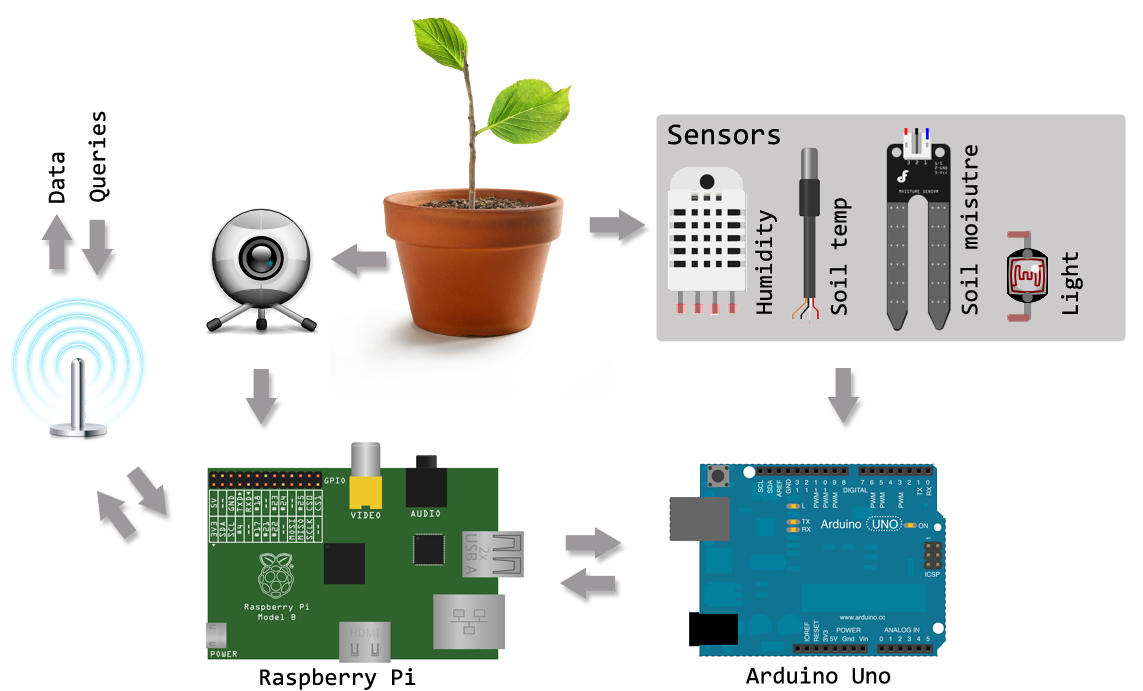
\includegraphics[width=1\textwidth]{img/hardware/application.png}
\caption{High-level illustration of the physical hardware components in the application}
\label{fig:application}
\end{figure}

\section{Plant data collection}
At the lowest level in the information hierarchy is the hardware and software responsible for capturing and uploading environmental data regarding the plant. Like a patient in a hospital, the plant is connected to a range of sensors, each responsible for reading a specific variable that is important for the plant's functioning. These variables are sent to a computer, processed, and uploaded to the next level in the data hierarchy. In the following sections we will follow the data on its way from the plant's physical location to the "cloud" and the user.

\subsection{Sensors}

\def\arraystretch{1.8}
\begin{table}
    \begin{tabular}{@{}lp{250pt}@{}}\toprule
    Sensor               & Description \\ \midrule                                                                                                  
    TSL2561              & Digital luminosity sensor. Measures light in lux from 300-1100nm.                                            \\ 
    RHT03                & Digital humidity and temperature sensor. Measures relative humidity and temperature in celsius.              \\ 
    DS18B20              & Digital waterproof temperature sensor. Measures temperature in celsius                                       \\ 
    DFRobot sku:sen0114  & Analog soil moisture sensor. Returns values between 0 and 900 depending on electrical conductivity of soil.  \\ \bottomrule
    \end{tabular}
    \caption{Sensors used in the application}
\end{table}


With the advent of the \emph{“internet of things”}, sensors are becoming available in many different forms and packages. Just as LEGO-pieces they are cheap and can be used as modular building blocks in a wide range of applications. From automating tasks such as keeping a steady indoor-temperature, to measuring variables that humans cannot see. 

The sensors are able to capture information concerning the environment and transform it to data variables, which we can store and categorize. In total there are five different sensors connected to the plant, or in the plant’s vicinity: soil moisture, soil temperature, air temperature, humidity, and light. 


%(write something about the sensortag)

The sensors we have used in this project are analogous to a volume controller on an amplifier. On an amplifier one can adjust the volume by varying the resistance in the signal going to the speakers. If we turn the volume up, the resistance goes down, and if we turn the volume down, the resistance goes up. Sensors work in the same way, but instead of controlling resistance with a volume knob, it is controlled by light, moisture or other environmental variables. 

To exemplify let's look at temperature sensors, or "thermistors". They vary their resistance in relation to the temperature. Since we already know how many volts we are sending to the thermistor on the one end, we can use the amount of volts we get back to calculate the resistance. In our application this is done by a voltage divider, which uses a formula as follows: 

\begin{equation}
U_{out}=\frac{R_{2}}{R_{1}+R_{2}}\cdot U_{in} 
\label{eq:vdiv1}
\end{equation}
Where $V_{out}$ is voltage out, $U_{in}$ is voltage in, $R_{1}$ is a given resistance, and $R_{2}$ is the resistance we want to calculate. For this example let's assume that $U_{in} = 5_{v}$, $U_{out} = 2_{v}$, and $R_{1} = 1K\Omega$. We solve this equation with regard to $R_{2}$
\begin{equation}
R_{2} = \frac{U_{out} \cdot R_{1}}{U_{in}-U_{out}}
\end{equation} 

\begin{equation}
R_{2} = \frac{2V \cdot 1000\Omega}{5V-2V}
\end{equation} 

\begin{equation}
R_{2} = \frac{2000\Omega}{3}
\end{equation} 

\begin{equation}
R_{2} = 667\Omega
\end{equation} 

Then we can see that the calculated resistance is 667$\Omega$. This value can then be mapped to the correct unit of measure, in this case Celsius or Fahrenheit. 

As we are using digital sensors, all of these calculations are done internally in the sensors, and coded into a digital signal. This signal, consisting of 1s and 0s, is then passed onto the next unit in our system, the Arduino.  

\subsection{Arduino}
%(Write about embedded systems. What other alternatives are there to the Arduino? )

Arduino is an open-source prototyping platform that makes it easy to interface low-level electronics (i.e sensors) with higher-level electronics (i.e computers). The core part of the Arduino is an Atmel\texttrademark Atmega microcontroller, which can be programmed by a computer over a USB port, using the Arduino programming language and the Arduino development environment \citep{Arduino}.

%We have used an Arduino Uno that has 13 digital input output pins (GPIO), five analog inputs, i2c inputs, and a USB port for serial communication. The soil temperature sensor and the temperature and humidity sensor are connected to the digital inputs through a 1K(ohm) pullup resistor. The pullup resistor is used to keep the voltage sent to the Arduino from fluctuating when the sensor is not sending any data. The TSL2561 luminosity sensor is connected to the A4/SDA and A5/SDL ports of the Arduino as it communicates over the i2c protocol. And the DFRobot soil moisture sensor is connected to A3 (Analog input 3) as it outputs analog voltage.  

\begin{figure}
\centering
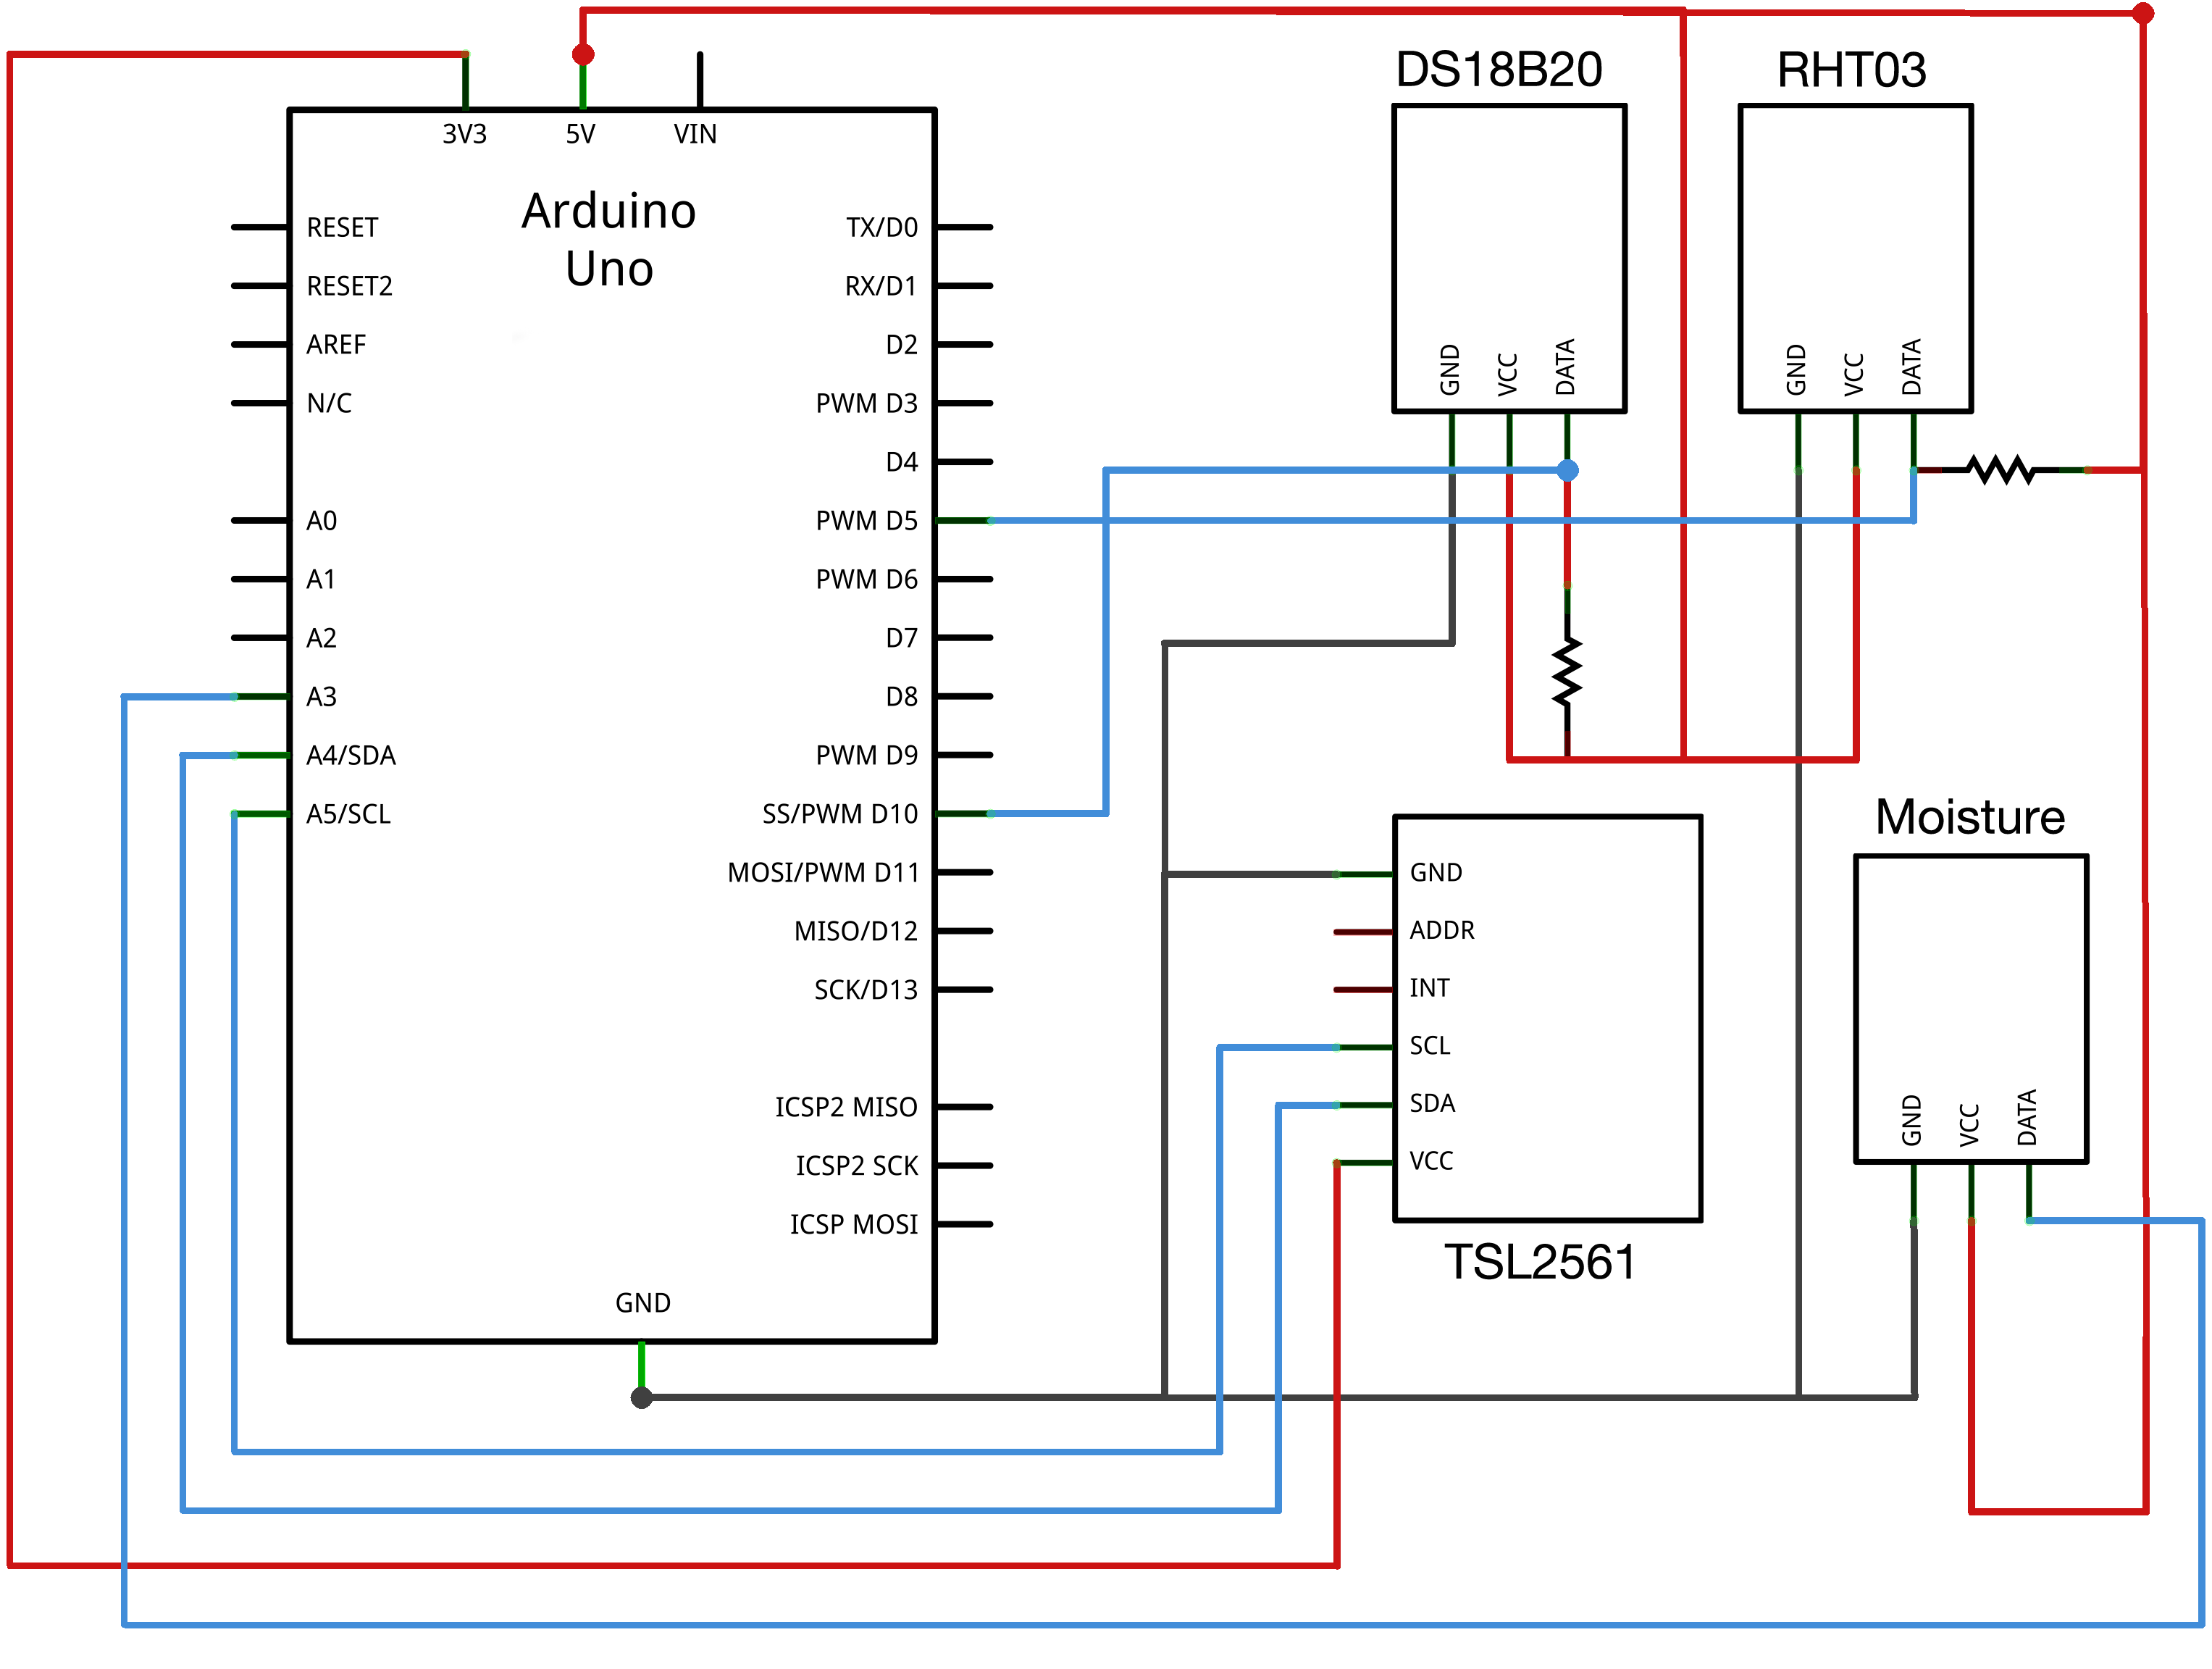
\includegraphics[width=1\textwidth]{img/hardware/Arduino_and_sensors_schem.png}
\caption{Schema diagram of Arduino sensor wiring. Pullup resistors on the data line of the temperature sensors. The TSL2561 light sensor communicates over the i2c protocol (SDA,SCL), and the soil moisture sensor connects to analog input}
\label{fig:Arduino}
\end{figure}

The community surrounding Arduino is quite large, and we have therefore been able to find pre-written libraries for communicating with the different sensors. This has simplified the task of converting the digital signal to the correct units (celsius, relative humidity, lux). 

In the case of the soil moisture sensor, it measures conductivity in the soil, and does not output moisture levels in any kind of universal measuring unit. But the conductivity measured in the soil is repeatable and proportional to the moisture level. Therefore we measured the resistance in air (high resistance), and in water (low resistance), and let these be the high and low points of a new unit called arbitrary moisture units (AMU) \citep{ch00ftech}.

The code residing in the Arduino runs a simple loop where it waits for a special character sent over serial communication through USB. If it receives this character it reads all the sensor values, and sends them back to the next logical unit in the Monoplant system: the Raspberry Pi

\subsection{Raspberry Pi}
%(Why Raspberry? Beagleboard?)
The Raspberry Pi is a “cheap, accessible, programmable computer” \citep{Raspberrypi}, which is roughly the size of a credit card. Our model was released in early 2012 and contains two usb ports, audio, sd-card slot, and several GPIO-pins. We have connected a wireless network adapter, a high-definition webcam, a powered USB-hub, and an Arduino to the Raspberry. The operating system running on it is a port of Debian Linux optimized for the Raspberry, called Raspbian. 

\begin{figure}
\centering
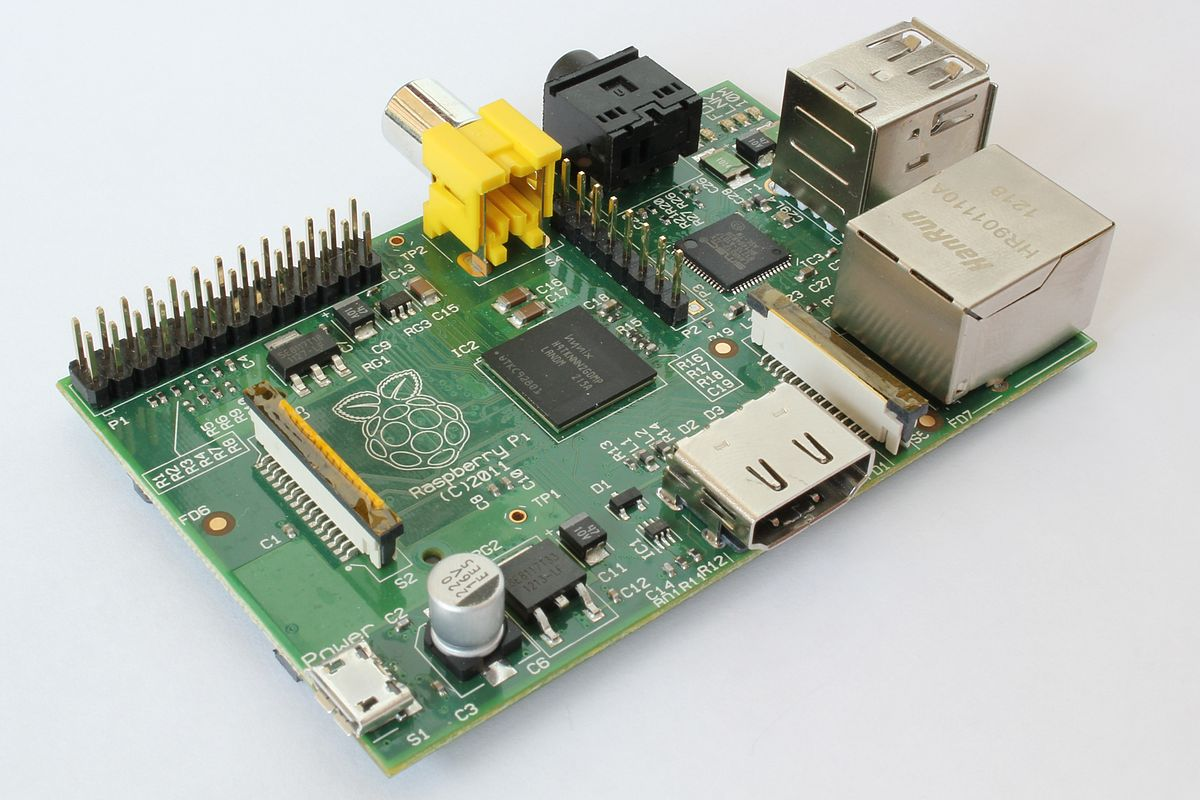
\includegraphics[width=1\textwidth]{img/hardware/1200px-RaspberryPi.jpg}
\caption{Raspberry Pi}
\label{fig:Raspberry}
\end{figure}

The GPIO-pins on the Raspberry works almost in the same fashion as the Arduino's digital input output pins. Thus we could in theory simplified the hardware by omitting the Arduino. The main reason for not doing this is that the Raspberry does not have an analog to digital converter (ADC). Therefore we would have to make a complex circuit involving an ADC to interface the Raspberry with the soil moisture sensor. In addition, we would most likely face timing issues. When we ask the digital sensors for data, they send the response immediately. If the unit receiving is not available to read the data, it gets lost. This can be a problem when using a high-level computer, as it performs multiple tasks in addition to reading sensordata. 

\subsubsection{Operation}
After booting up, a bash-script with an endless loop is called. The script snaps a photo of the plant using the webcam, and then runs a python-script responsible for collecting sensordata. Since we sometimes can get erroneous values from the sensors, we read 15 values and upload the median value. These values, along with the photo captured by the webcam, are then passed on to the next logical unit in the Monoplant system. 

%http://en.wikibooks.org/wiki/LaTeX/Packages/Listings
\lstset{language=Python} 
\begin{figure}
\begin{lstlisting}
//instantiate lists
airtemp = []
humidity = []
light = []
soiltemp = [] 

for x in xrange(1,15): 
	ser.write("r") //Ask Arduino for data
	variables = ser.readline() //Read the data
	sensorReadings = variables.split('|') //Split string on |

	airtemp.append(float(sensorReadings[0]))
	humidity.append(float(sensorReadings[1]))
	light.append(float(sensorReadings[2]))
	soiltemp.append(float((sensorReadings[3])[:-2])) 

//calculate and post the median using numpy
postData(np.median(airtemp),np.median(humidity),np.median(light),np.median(soiltemp)) 
\end{lstlisting}
\caption{Reading sensor values from Arduino on Raspberry Pi, written in Python}
\label{fig:Raspberrycode}
\end{figure}

\section{Data processing and database}
When the data has been gathered at the low level hierarchy, it is stored in the cloud. This is done by posting the data to an application programming interface (API) on our web server. The main function of an API is to be a means of communication between different software, in our case the data collector and the user interface. After some research on web-API design, we decided that a REST architectual style was best suited for our application. 
%REST uses URIs and HTTP by default, the data you send is the data you send. This meas that the data is easy to use out of the box, 
%SOAP can use URIs and HTTP, the data you send becomes larger as verbose SOAP-standards are added to the data.

\subsection{Representational State Transfer (REST)}
REST is an architectual style for distributed hypermedia systems \citep{fielding2000architectural}. In Fielding's dissertation, he writes about the interaction constraints of REST that is introduced in order to limit how a distributed system can be constructed. 

\begin{enumerate}
\item{} \emph{Client/Server} - This constraint separates the concerns of the client and the server. By separating these concerns, one secures that the two can evolve independent of each other. The client does not care about the internal logic of the server, and the server does not care what the client does with the data. This gives us the ability to separate the concerns of data collection, data storage and data visualization, which gives us the freedom to change the internal logic of any one of these without worrying about breaking the other two. It also means that we can create several different clients either for collecting data or displaying data.

\item{} \emph{Stateless} - The communication between client and server must be stateless. The request from client to server must contain all the information needed to understand the request. In practice this gives the client the responsibility to keep track of the state.

\item{} \emph{Caching} - In order to reduce requests and improve efficiency, the server can state which responses can be reused by the client when sending equivalent requests. This can greatly enhance user-perceived performance, but at the same time reduce reliability if cached data differs from what would have been delivered by the server on a request. We could theoretically cache almost everything since our data belongs to specific timestamps, and the chances that a sensor value is updated at a later time is minimal. However, since we are developing a prototype and have the need for rAPId changes in the implementation, we have experienced that the need for reliable data exceeds the need for fast performance.

\item{} \emph{Uniform interface} - This is a rather complex constraint in terms of RESTful API design, and is the reason for a lot of discussions around implementation of true REST. Fielding describes a REST interface to be:

\begin{quote} efficient for large-grain hypermedia data transfer, optimizing for the common case of the Web, but resulting in an interface that is not optimal for other forms of architectural interaction. \citep{fielding2000architectural} 
\end{quote}

In an applied context this means that the server has resources that can be referenced via URLs and operated through the HTTP-verbs. In order to be a true REST interface, an API can have any resource available through URLs, but the only methods in which one can operate the resource is POST, GET, PUT and DELETE.

\item{} \emph{Layered system} - This constraint tells us that a REST interface may hide complexity hierarchically, by masking information so each component cannot "see" beyond the immediate layer with which they are interacting. \citep{fielding2000architectural}

\item{} \emph{Code on demand} - An optional constraint, allowing the server to serve executable code to the client. 

\end{enumerate}

REST is an architectual style, not a strict standard. It allows for flexibility, but at the same time promotes best practice. The goal of our API was to provide a way of storing and accessing plant data in the cloud, first and foremost for client side applications that we built ourselves. Our objective was to create something that worked for us. A pragmatic approach to REST gave us the flexibility to create an API that gets the job done. In the following chapter we will describe how the API works and discuss some choices we made in the implementation process.

\subsection{Application Programming Interface - API}
Our first implementation of the API was written in PHP with the framework Codeigniter. This worked well for a while, but after having made several dirty hacks and workarounds we decided to look for other options. After researching Ruby on Rails and their focus on "convention over configuration", we found that it was a framework well suited for building our API.  

\begin{quote}
Ruby on Rails is an open-source web framework that’s optimized for programmer happinees and sustainable productivity. It lets you write beautyful code by favoring convention over configuration. \citep{rubyonrails.org} 
\end{quote}

Ruby on Rails (RoR) makes the assumption that there is a "best" way of doing things, and encourages that way. It emphasizes well-known software engineering principles such as convention over configuration, don't repeat yourself, model-view-controller and REST.

Our web server is running on Amazon Elastic Compute Cloud (ec2), a virtual computer service with low costs and extensive configuration options. We chose this because we needed to be able to configure the server for our purposes and install several libraries and applications onto the server. 
%We wanted to create the API The API is created with Ruby on Rails to 

Our API is a server-side Web-API that can be accessed through the HTTP-protocol. To use it, one can send a request to the domain of the API from any client that can send HTTP-requests. The API will interpret the request and respond based on how the interpretation went. Since our API is based on the REST architectual style, it adheres to how the HTTP-protocol is built, meaning that a resource has a unique identifier, a URI, and some uniform actions called the HTTP-verbs which the resource can be operated with. There are 8 methods in the HTTP/1.1 protocol \citep[p.36]{fielding1999hypertext}, but only four of them are of interest when speaking of resources. These methods are the four basic functions of persistent storage in computer programming, often referred to as CRUD (Create, Read, Update and Delete), but in HTTP their names are POST, GET, PUT and DELETE. 

The Monoplant API have three resources: Plants, Sensorvalues and Videos. To create a plant, one can send a POST request to the URL: \begin{verbatim}http://Monoplant.me/plants.json\end{verbatim} A post request also needs information about the plant to create, in this case we will pass that information in the json-format:

\begin{figure}[H]
	\begin{lstlisting}[language=javascript]
	 {"plant": {"name": "Alfa", "location": "Intermedia", "plant_type": "Alfalfaspire"}} 
	\end{lstlisting}
	\caption{POST plant json data}
	\label{fig:postdata}
\end{figure}

For the API to know how to interpret this information in json, we also need to pass a parameter in the header called Content-type, this variable will be set to “application/json”. When we pass this request, the API will create a plant with the information we gave it, and give a response with the code: \verb@"201 created"@. The response contains a header and a body in which the header has some meta-data about the request and the body will contain a representation of the created plant (see figure~\ref{fig:plantresponse} on page~\pageref{fig:plantresponse}).

\begin{figure}
	\begin{lstlisting}[language=javascript]
	{
		created_at: "2013-09-17T10:45:17+02:00"
		id: 1
		location: "Intermedia"
		name: "Alfa"
		plant_type: "Alfalfaspire"
		updated_at: "2013-09-17T10:45:17+02:00"
	}
	\end{lstlisting}
	\caption{Plant response in json}
	\label{fig:plantresponse}
\end{figure}

If we look at this representation, we see that the API has added an ID to the plant as well as two data attributes created\_at and updated\_at. Since we now have the id of the plant, we can tell the Raspberry Pi to start adding sensor values for that specific plant. The Raspberry will create a request using the data it gets from the Arduino and the image from the webcam and finally send that POST request to the URL:\begin{verbatim}http://Monoplant.me/plants/1/sensorvalues.json \end{verbatim}

As in the first example the API will interpret the request, store the data, and respond with a status code: \verb@"201 created"@. In the background, the API will generate a thumbnail of the image and upload both the thumbnail and the original to another static server, finally storing the URL for both of them in the database. The response body ends up looking as shown in figure~\ref{fig:sensorvaluesresponse}. If we need to look at this sensorvalue at a later time, we can simply do a GET request using the sensorvalue id we got from the previous response and call the URL:\begin{verbatim}http://Monoplant.me/plants/1/sensorvalues/10037.json \end{verbatim} This will make the API respond with a status code \verb@"302 Found"@, and the body will look just like the previous response body, unless it has been updated in the meantime. Note that the URL is built up according to which resource we are trying to operate. See table~\ref{fig:RESTurl} for an overview of how these URLs are built up.

Now that the data from the plant is securely stored in a database and accessible through the API, we move on to how these data are further processed to generate timelapse videos. 

\begin{figure}
    \begin{lstlisting}[language=javascript]
    {
        airTemp: 22.14
        created_at: "2013-09-17T10:49:43+02:00"
        humidity: 38.5
        id: 10037
        img_url: "http://s3-eu-west-1.amazonaws.com/plantespann/2013/9/17/original/10037.jpg?1379407782"
        light: 1702.5
        photo_content_type: "image/jpeg"
        photo_file_name: "viewcam.jpg"
        photo_file_size: 204358
        photo_updated_at: "2013-09-17T10:49:42+02:00"
        plant_id: 1
        soilMoisture: 54
        soilTemp: 22.25
        thumb_url: "http://s3-eu-west-1.amazonaws.com/plantespann/2013/9/17/thumb/10037.jpg?1379407782"
        updated_at: "2013-09-17T10:49:43+02:00"
    }
    \end{lstlisting}
    \caption{Sensorvalues response from Monoplant}
    \label{fig:sensorvaluesresponse}
\end{figure}



\bgroup
\def\arraystretch{1.8}	%  margin for cells 1 is default
\begin{table*}
	\centering
	\begin{tabular}{@{}lp{250pt}@{}} \toprule
		\textbf{part of URL}&	\textbf{meaning}\\ \midrule
		\texttt{http://}&	the protocol we acces the API through\\ 
		\texttt{Monoplant.me}&	the domain of the API\\ 
		\texttt{/plants/(:id)}&	\texttt{/plants} states that we want to access a resource named plant \\ &
		\texttt{/(:id)} is a number representing the specific plant we want to access\\ 
		\texttt{/sensorvalues/(:id)}&	\texttt{/sensorvalues} states that we want to access a resource named sensorvalue. Since this comes after \texttt{/plants/(:id)} it means that we will get sensorvalues owned by the plant with \texttt{(:id)}. \\ &
		\texttt{/(:id)} is a number representing the specific sensorvalue we want to access\\ 
		\texttt{(.format)}&	 \texttt{.format} can be blank, .html, .xml or .json. If it is blank, the API will respond with the default format, in our case html. If not it will respond with the corresponding format.\\ \bottomrule
	\end{tabular}
	\caption{How a REST-url is built up}
	\label{fig:RESTurl}
\end{table*}
\egroup

\subsection{Generating timelapse videos}
Regular video cameras capture 24 to 30 images or frames per second (fps), and play them back at the same rate. The events in the video will then unfold at the same speed in which they happened during the shoot. Timelapse photography utilizes this principle by slowing down the rate at which images are captured, while maintaining the playback rate. So for instance if we captured one image per second, and played it back at 24 fps, one second in the film would equal 24 seconds in real life. Thus when played back, time would appear to move faster. This makes it possible to pronounce changes which are subtle to the human eye. E.g, a sunset, moving clouds, or a plant growing.  

Each day at midnight the system collects all the images taken during the day, and combine them to a timelapse video played back at 30 frames per second. As the Raspberry Pi captures approximately one picture per minute, one second in the video equals 30 minutes in real life. One picure each minute equals \begin{math} 60min*24hours=1440 \end{math}
pictures each day, which, if we divide it by 30 frames per second gives us a 48 second video representing 24 hours in real life. This equals a speed increase of 1800 times. 

%Logically, to adhere to the principle of separation between data generation, storage and presentation. The Raspberry would generate the timelapse videos itself, and then push them to the API. But in an effort to reduce the amount of load on the Raspberry Pi, we decided to compile the timelapse videos needed on the same server as the API. By doing so the amount of data transferred from the PI to the API is also reduced, as the API server already has the processing power and the images needed for the generation. 

\subsubsection{HTML5 Video Element}
Prior to HTML5 there was no standard way of implementing videos on web-pages. Therefore the web was filled with a myriad of different solutions, with QuickTime, RealPlayer, and Flash being the most prominent \citep{pilgrim2010html5}.

In HTML5 we have a new, standard \verb@<video>@ element that in theory should give us support for native video in all browsers. But due to the nature of video-files, problems arise when users have different operating systems and different browsers. To be able to explain these problems, we a look at the architecture of a video file.

A video file consists of a container, a video codec, and audio codec. The container defines how the content within is stored, the video codec defines how the video stream is encoded, and the audio codec defines how the audio is encoded. Since there exists numerous containers, video- and audio codecs, endless permutations are possible. Therefore it is not likely that we will have a combination that would work in all browsers in any foreseeable future \citep{pilgrim2010html5}.

In order to maximize compatibility in our application, we decided to encode video in three different formats: H.264+MP4, Webm and Theora (see table~\ref{tab:videosupport}). This is done via a bash script that runs every night. First, we run a perl script for "deflickering", i.e calculate and convert the images to a median brightness to reduce video flickering. Then we use the programs Mencoder and FFmpeg2theora to create H.264-, webm- and theora-videos. And finally, the videos are posted to the respective plants in the database, using the API. 

After the data has been collected from the sensors and uploaded through the API. And we have generated timelapse videos in different formats. We are ready for the next logical unit in the Monoplant application, displaying information to the users. 

\begin{table*}\centering
\begin{tabular}{@{}lcccc@{}} \toprule
Codecs/containers & IE & Firefox & Safari & Chrome \\ \midrule
Theora+Vorbis+Ogg & ~                 & 3.5+    & ~      & 5.0+   \\ 
H.264+AAC+MP4     & 9.0+              & ~       & 3.0+   & 5.0+   \\ 
WebM              & 9.0+              & 4.0+    & ~      & 6.0+   \\ \bottomrule
\end{tabular}
\caption{Video support in different browsers \citep{pilgrim2010html5}}
\label{tab:videosupport}
\end{table*}

%http://en.wikibooks.org/wiki/LaTeX/Packages/Listings
% \lstset{language=bash} 
% \begin{figure}
% \begin{lstlisting}
% #!/bin/bash
% #get yesterdays date
% year=`/bin/date -d '1 day ago' +%Y`

% date=`/bin/date -d '1 day ago' +%m`
% month=`expr $date + 0`

% date=`/bin/date -d '1 day ago' +%d`
% day=`expr $date + 0`

% #copy files
% cp /mnt/s3/plant_2/$year/$month/$day/original/* /home/ubuntu/bin/timelapse/source_folder_of_pictures/

% #run deflicker
% perl /home/ubuntu/bin/timelapse/timelapse-deflicker.pl

% #step into deflickered folder
% cd /home/ubuntu/bin/timelapse/source_folder_of_pictures/Deflickered

% #get a file for the coverpicture
% ls | grep -v files.txt > files.txt 
% coverpicture=$(sed -n '100p' < files.txt)
% rm files.txt

% #create video h264
% /usr/bin/mencoder -idx -nosound -noskip -of avi -ovc x264 -x264encopts pass=1:bitrate=2000:crf=24:bframes=0 -o output.avi -mf fps=30 'mf://@files.txt'
% /usr/bin/MP4Box -aviraw video output.avi
% /usr/bin/MP4Box -add output_video.h264 output.mp4

% #create video theora (ogv)
% /usr/local/bin/ffmpeg2theora --noaudio -v 7 output.avi

% #create video webm
% /usr/bin/mencoder -idx -ovc lavc -nosound -of lavf -lavfopts format=webm -lavcopts threads=4:vcodec=libvpx -ffourcc VP80 output.mp4 -o output.webm

% \end{lstlisting}
% \caption{Video encoding for HTML5}
% \label{fig:videoencoding}
% \end{figure}

\section{User Interface}
The user interface (UI) of Monoplant is where we visualize the data from the API to the users. It is accessible through web, and displays correctly on most devices due to a responsive design. The UI is built with RoR as web application framework, Bootstrap as design framework, and Highcharts as graph framework.   

The main page of each plant represents the current state of the plant. On the left side, it displays the last picture with the corresponding temperature, humidity, light and soil moisture. On the right side, there is a timelapse video from the day before, with a corresponding graph displaying all the sensorvalues throughout that day (see figure~\ref{fig:mainpage} on page~\pageref{fig:mainpage}). 

On the top of the page there are two menu items. The first  is called "videos" and links to the video overview. This is a page containing all the videos for the plant selected. In relation to each video, the max and min values for all the different sensors during that day is shown. The second menu item is called "graphs" and is a drop-down menu with links to graphs for each of the different sensors. In addition there is a link to the graph containing all the sensorvalues for the last 24 hours. 

During our work with the UI, there was two aspects that proved to be particularly challenging: relative graphs, and connecting the timelapse videos to the graph. In the following sections the work with these obstacles will be explained. 

\begin{figure}
\centering
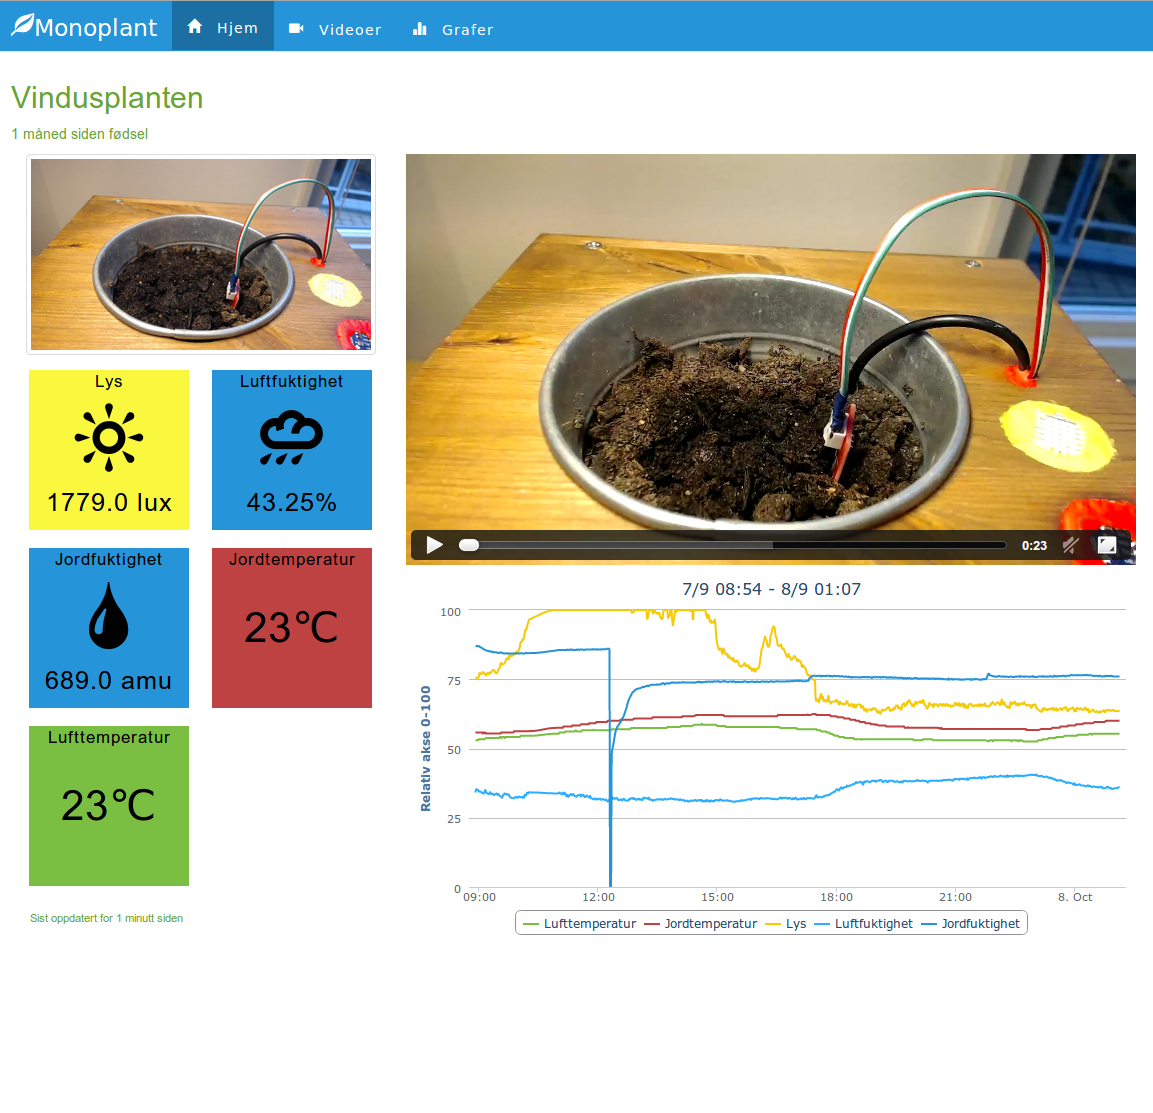
\includegraphics[width=1\textwidth]{img/interface/mainpage.png}
\caption{Screenshot from user interface}
\label{fig:mainpage}
\end{figure}

\subsection{Highcharts}
There are 4-5 serious javascript chart libraries on the Internet with various types of focus, flexibility and documentation. We ran some tests with Google charts, d3.js and Highcharts, and found that Highcharts provided the most extensive documentation as well as an easy to understand interface. 

The first graph we had to make was a graph containing all the plant data from a given time corresponding to the timelapse video. This meant putting temperature, light, humidity and soil moisture in the same graph, even though they all have different units. 



\begin{figure}
\centering
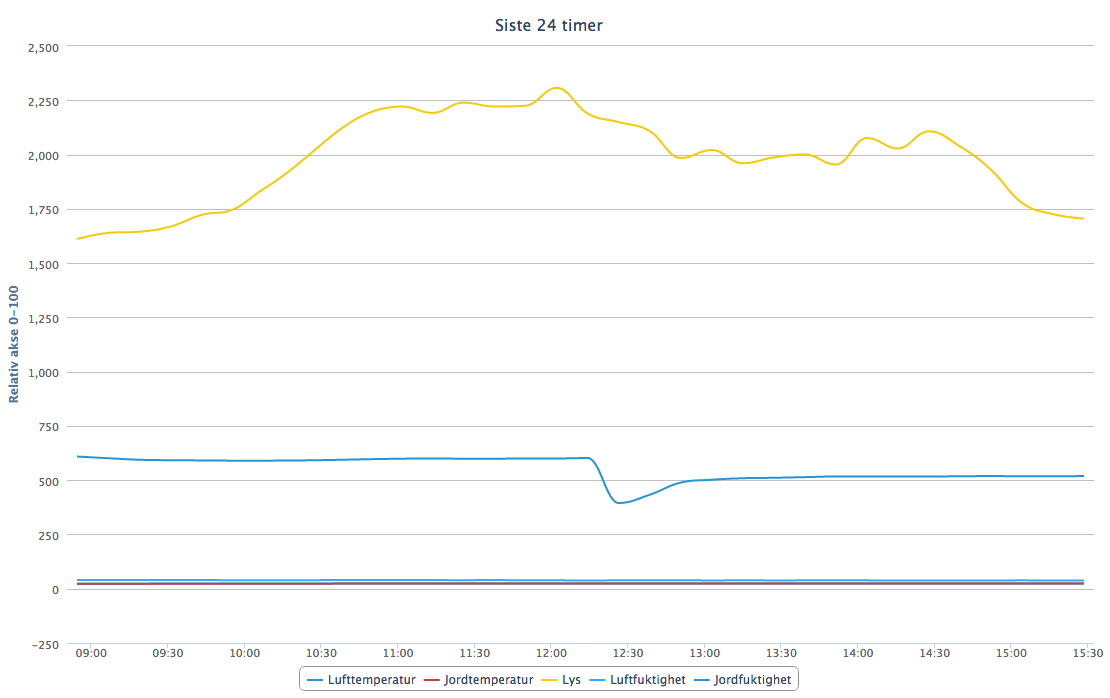
\includegraphics[width=1\textwidth]{img/interface/badgraph.png}
\caption{Screenshot from an unsuccessful graph}
\label{fig:badgraph}
\end{figure}

Our first attempt was done without manipulating the data at all. As Highcharts scales the chart based on the element with the largest numbers and changes, the element with small numbers and changes appeared as straight lines at the bottom of the graph. In figure~\ref{fig:badgraph} we tried to combine light levels of 2000 lux with temperature levels at $22\,^{\circ}\mathrm{C}$, and as we can see, all the elements except light and humidity are concentrated at the bottom. 

For this graph to display the environmental changes during a day we needed to create a relative scale and map the values to that scale. To exemplify, lets say you have a number X, which has a value between A and B, and you want to map it to a value Y, between C and D. The function can then be written as: 
\begin{equation}
Y = \frac{(X-A)}{(B-A)} * (D-C) + C
\end{equation}

%This becomes a slightly more advanced version of calculating percentage (see figure~\ref{fig:mapfunc} on page~\pageref{fig:mapfunc}).

%We chose an output scale from 0 to 100 and wrote a function according to figure~\ref{fig:mapfunc} that mapped the values based on what type of data it was. We set the input scales as can be seen in figure~\ref{fig:mapscale}.

\begin{figure}[H]
	\begin{lstlisting}[language=javascript]
	humidity: { min: 10, max:100 },
	soil temprature: { min:15, max:30 },
	light: { min: 400, max:2500 },
	air temprature: { min: 15, max: 30 },
	soil Moisture: { min: 0, max: 700 }
	\end{lstlisting}
	\caption{Mapping scales}
	\label{fig:mapscale}
\end{figure}

Through trial and error, we chose the \verb@C@ and \verb@D@ values of each unit (see figure~\ref{fig:mapscale}). Then, after running the data through our new function all the units became visible (see figure~\ref{fig:goodgraph} on page~\pageref{fig:goodgraph}). As we have mapped all the units to relative units, information of the values at the specific data points are lost. But as the graph is displayed along with the video, we wanted to keep the information level low.  

\begin{figure}
\centering
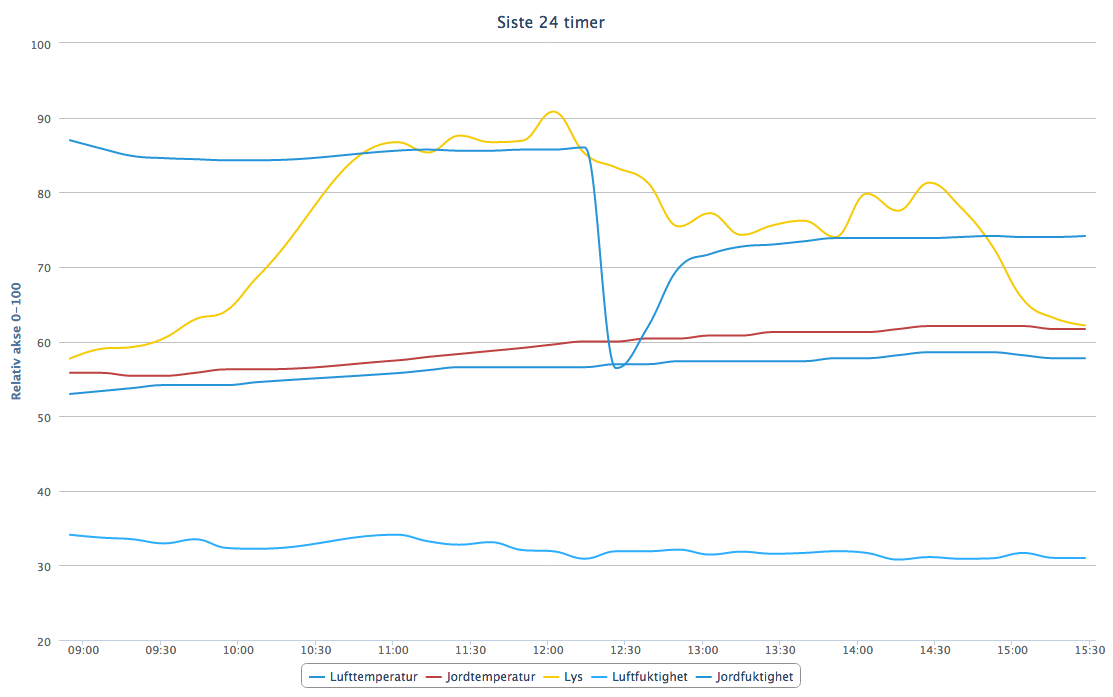
\includegraphics[width=1\textwidth]{img/interface/goodgraph.png}
\caption{Screenshot from a succesful graph}
\label{fig:goodgraph}
\end{figure}

%To make sure one can read the appropriate sensorvalues we provide several other graphs, one for the last 24 hours, very similar to the video graph. The only difference is that we have included a mouse-over interaction technique with a tool-tip that displays the actual values alongside the corresponding image of the plant \citep[p.254]{kluge2010simulation}.

Apart from the video-graph and the last 24 hour-graph we provide singular line graphs for each variable, this gives us the ability to display graphs with correct y-axises. The user can select time period for these graphs by interacting with the small graph on the bottom. 

\subsection{Connecting video and graph}
%explain objective
In order to present how changes in sensor variables manifested themselves physically in the plant, we wanted to connect the graph and the timelapse video. The visual solution became to present the video above the graph, both contained within the screen. As the video is playing, a vertical line layered above the graph moves from left to right representing where we are in the video. 

The HTML5 video-element can be accessed through javascript, and by checking the state of the video we are able to make the Highcharts graph follow the video based on the currentTime of the videoelement.

\begin{figure}
	\begin{lstlisting}[language=javascript]
	function startVideo(){
	     interval = setInterval(function() {
	         var curtime = video.currentTime.toFixed(2);
	         if(curtime!= lastcurtime){
		 lastcurtime = curtime;
		 curmarker = Math.round(curtime*30);
		 stepTooltip(curmarker);
	         }
	     }, 33);
	}

	function stopVideo(){
		clearInterval(interval);
	}
	\end{lstlisting}
	\caption{Video and graph connection code, written in javascript}
	\label{fig:videocode}
\end{figure}

By binding startVideo() to the play-event of the video-element and stopVideo() to the pause and stop event, we are able to move the graph marker as the video plays. The reason for using \emph{setInterval} instead of the videos built-in event \emph{timeupdate} is that it is not specified how often the event will fire, but by testing we found that it was somewhere between 3-7 times per second, varying randomly from second to second. This was not often enough as the video had a framerate of 30 frames per second, which meant updating the graph at 1/10 of the speed of the video, resulting in a laggish experience of the graph. We experienced that using \emph{setInterval} gave use much more accuracy when setting it to run every 33th millisecond. No browsers guarantee that the performance of \emph{setInterval} will be faster than 50 ms, but by running tests \citep{adequatleyqood}, we found that the Chrome browser ran this on an average of 4.5 ms. Even though this can be slower when considering the load on the browser when playing a video, we found that in practice most browsers were able to play the video and update the graph simultaneously. 
